\chapter{The LHC-ATLAS Experiment}
\section{Large Hadron Collider}
\begin{figure}[tbp]
\begin{center}
%\subfigure[]{
 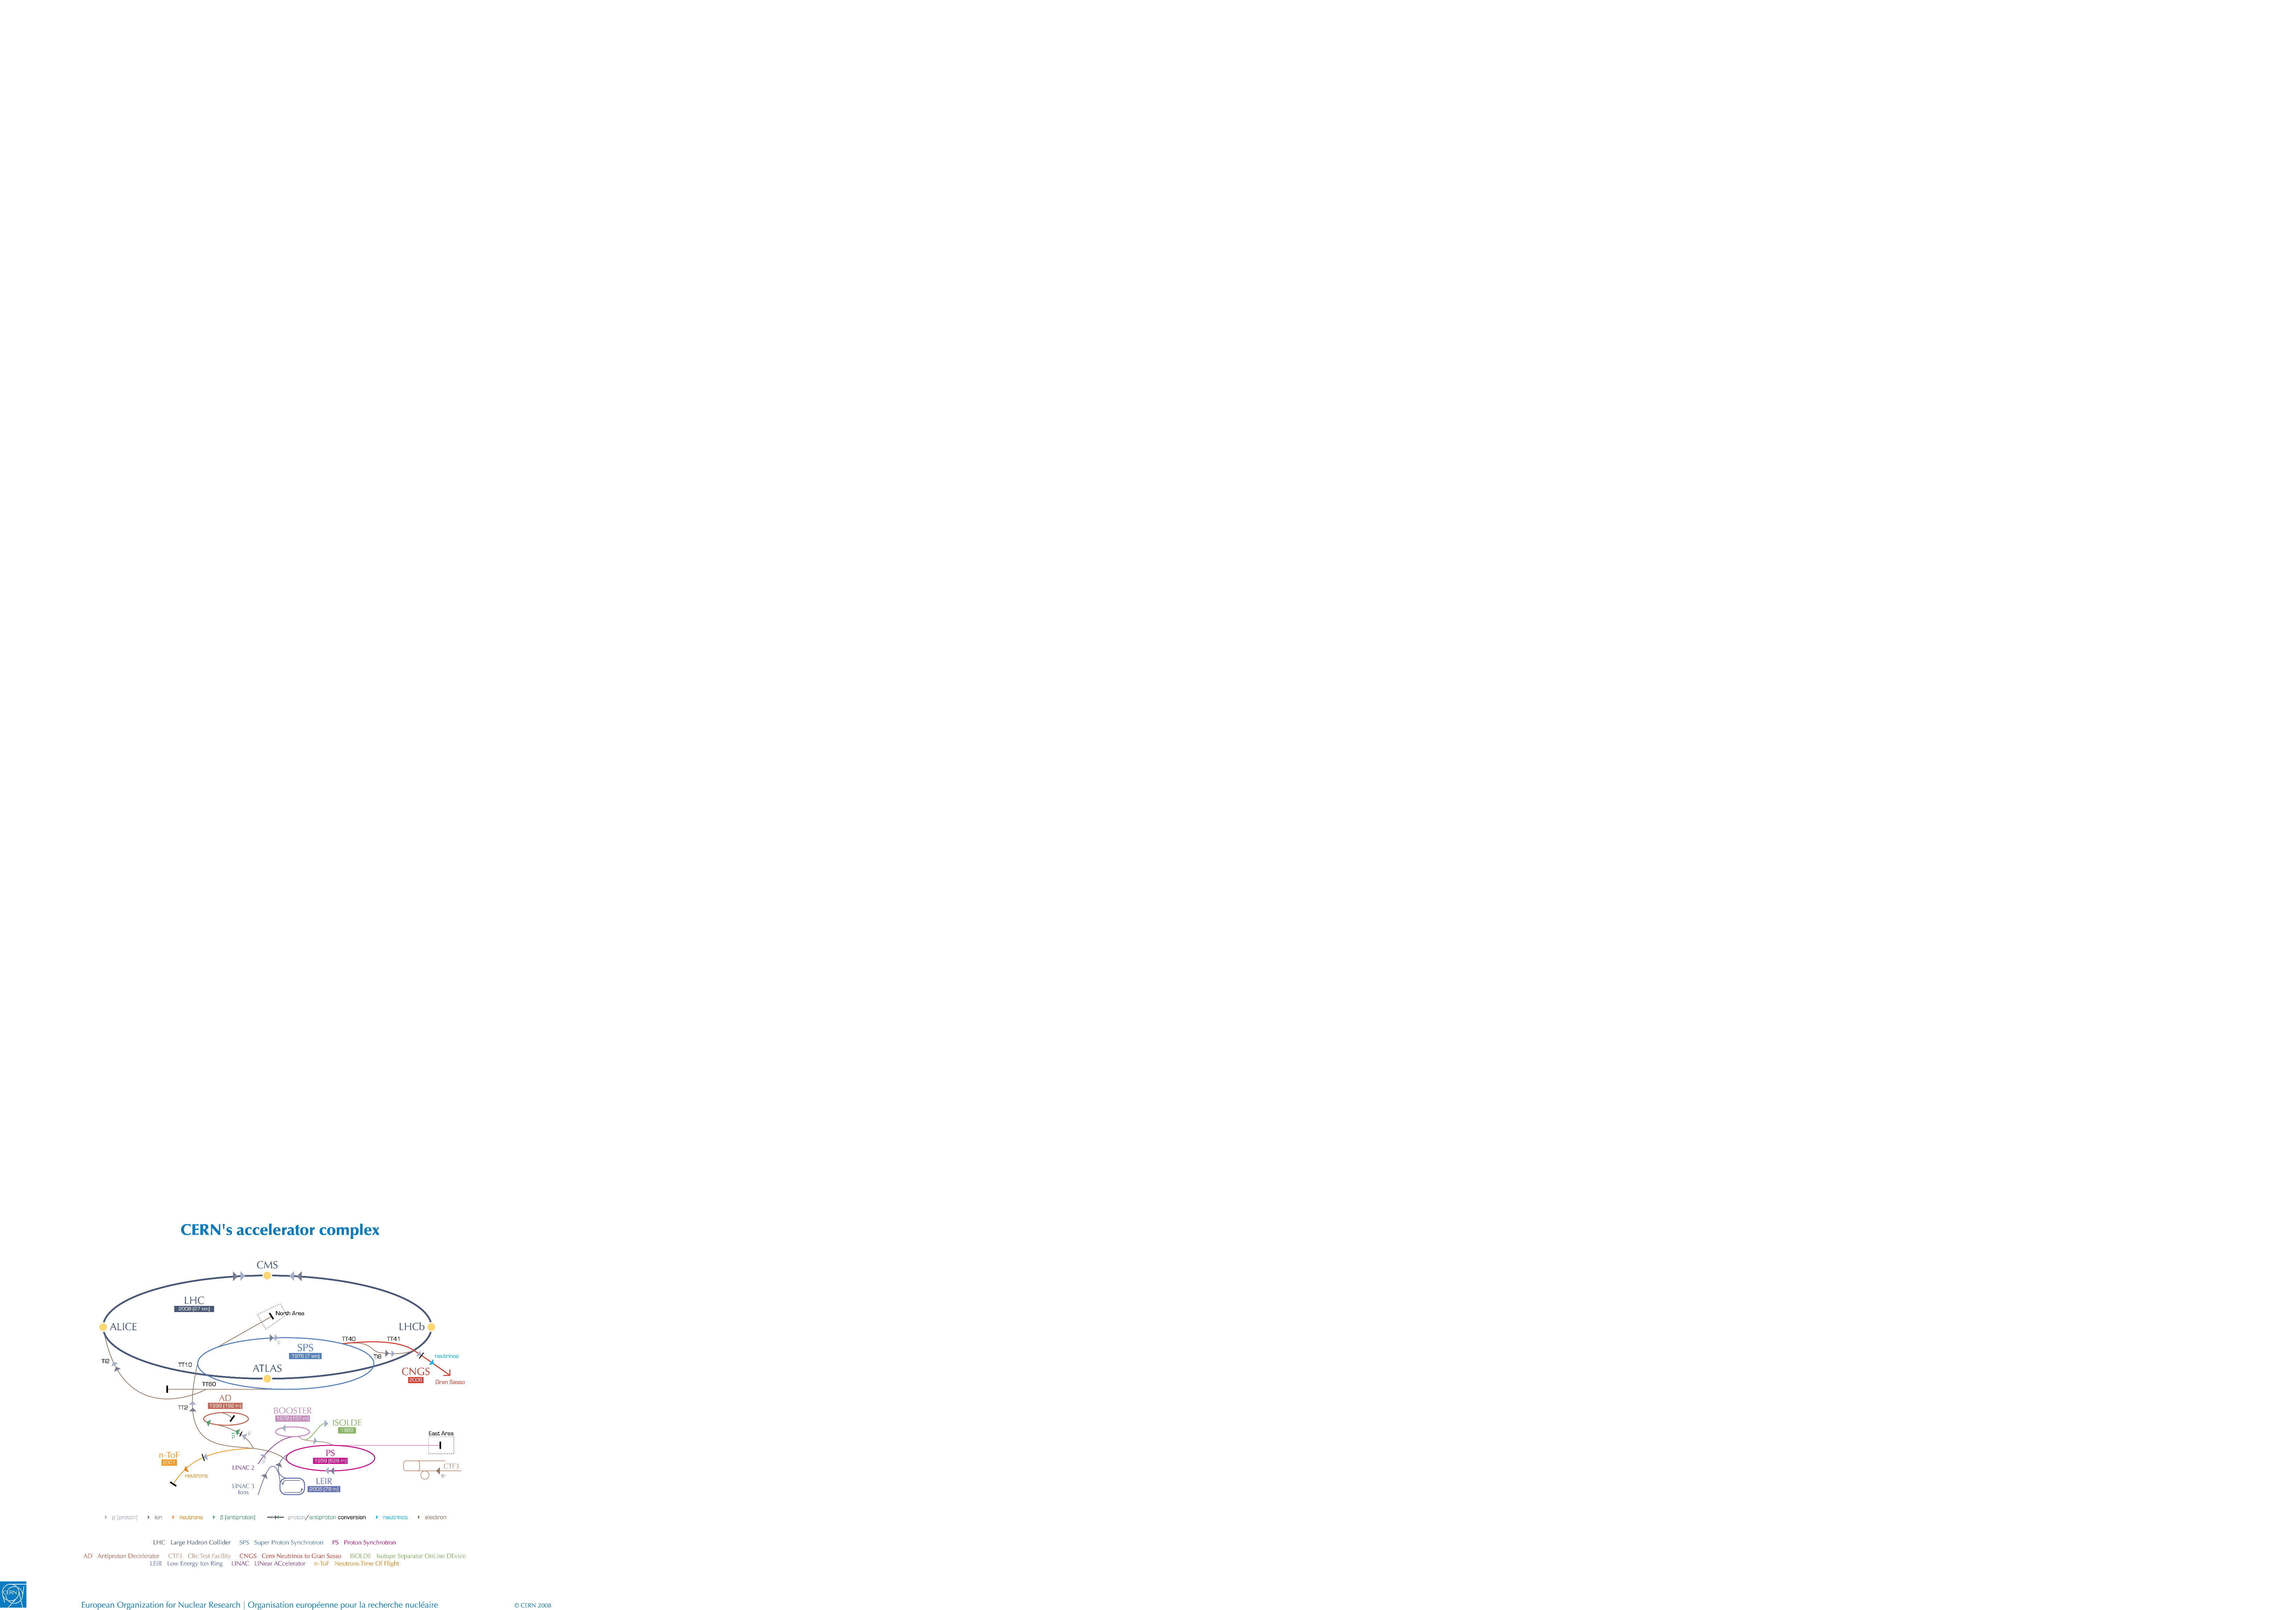
\includegraphics[width=1.0\textwidth,keepaspectratio]{figures/detector/CERN}
%}
\caption{
The whole picture of the CERN accelerator complex
}
\label{fig:CERN}
\end{center}
\end{figure}

\section{ATLAS Detector}
The ATLAS Detector [11] was designed to measure all standard model particles 2) produced by LHC collisions, a schematic overview of the whole ATLAS detector is shown in Figure 3.2. The detector position surrounding the beam pipe called barrel, and those aligned at the high η regions are referred to as end-caps.
The magnet system and the luminosity detector are introduced in Section 3.3.1 and 3.3.2, respectively. Four major subsystems, the inter tracker, the calorimeters, the muon spectrometer, and the trigger & data acquisition system are described.
\begin{figure}[tbp]
\begin{center}
%\subfigure[]{
 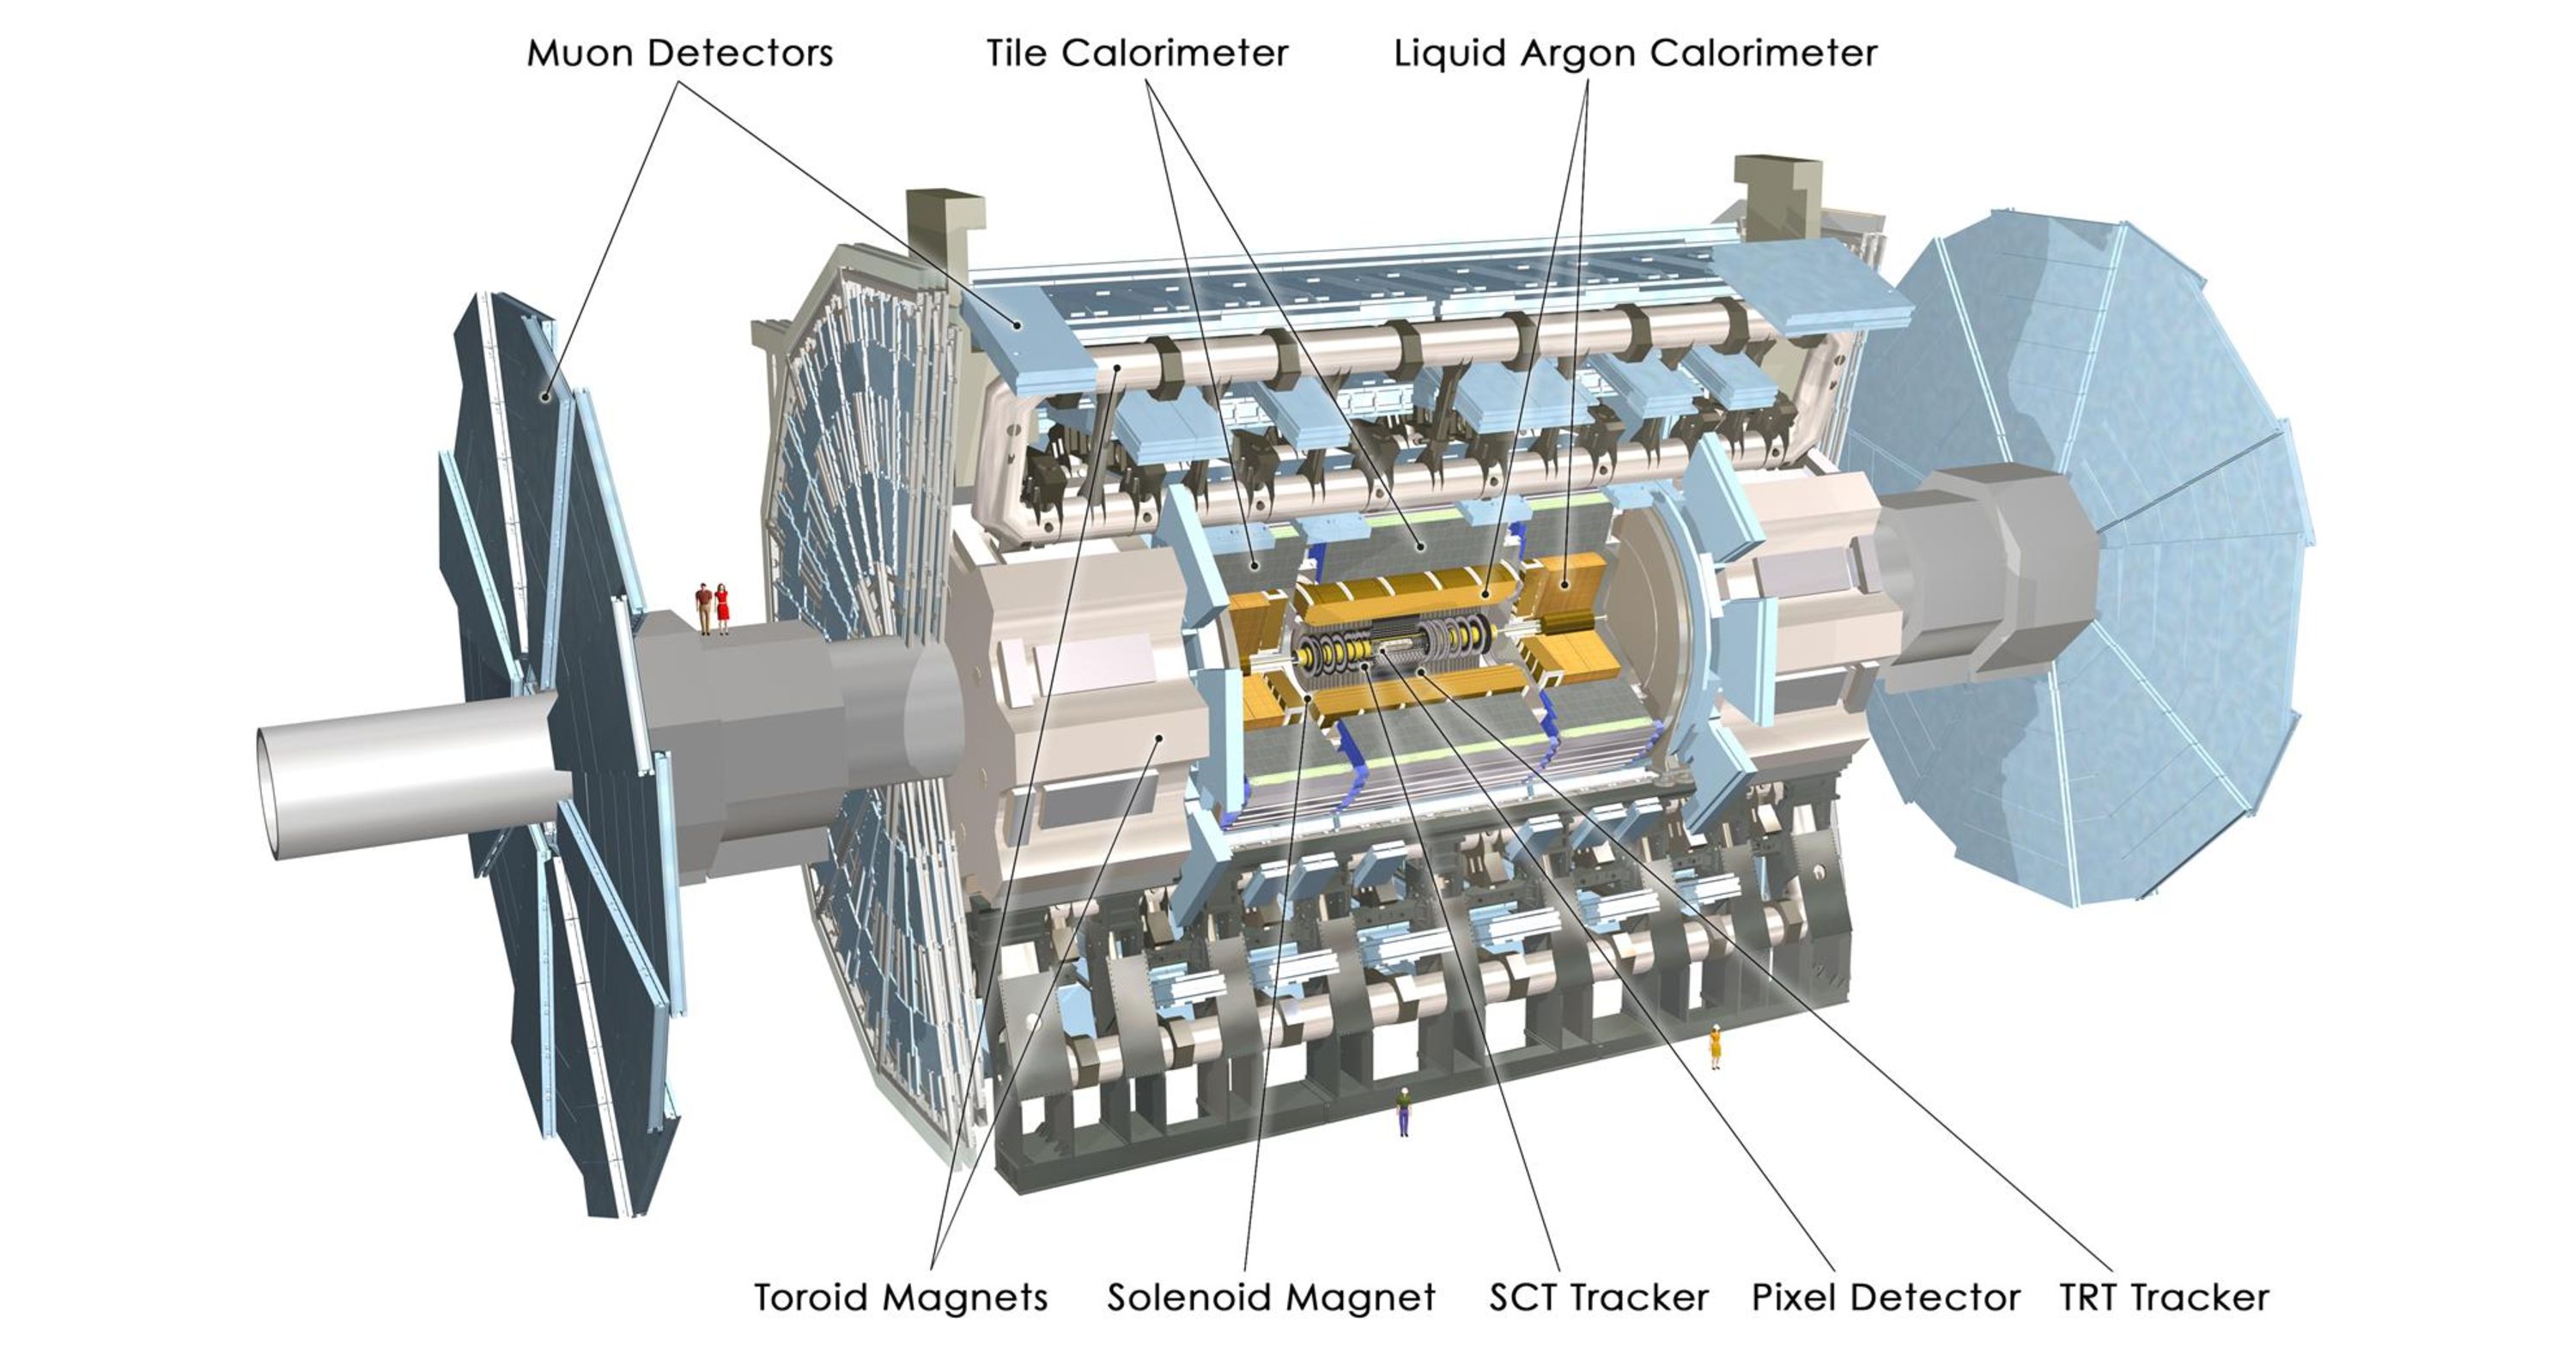
\includegraphics[width=1.0\textwidth,keepaspectratio]{figures/detector/ATLAS}
%}
\caption{
The whole picture of the ATLAS detector
}
\label{fig:CERN}
\end{center}
\end{figure}

\subsection{Magnet}
The ATLAS magnet system consists of four large superconducting magnets with a dimension of 22 m in diameter and 26 m in length with a stored energy of 1.6 GJ. A solenoid aligned on the beam axis generates 2 T axial magnetic field for the inner detector, which placed inside the calorimeter system. A toroid on the barrel and two toroids on the end-caps are installed and those provide 0.5 and 1T magnetic fields for muon detectors, respectively.
\subsection{Inner Tracker}
\subsubsection{Pixel Detector}
\subsubsection{SCT Detector}
\subsubsection{TRT Detector}
\subsection{Calorimeters}
\subsection{Muon Spectrometer}
\subsection{Trigger and Data Aquisition System}